
% Третья глава работы 
\chapter{Моделирование систем с алгоритмом RED в NS-2 и Mininet}
\label{chap3}

В данном разделе представлены результаты исследований. Для запуска моделей используем сеть c топологией, представленной в ~\ref{ch3:fig1}.
 
\begin{figure}[h!]
 \centerline{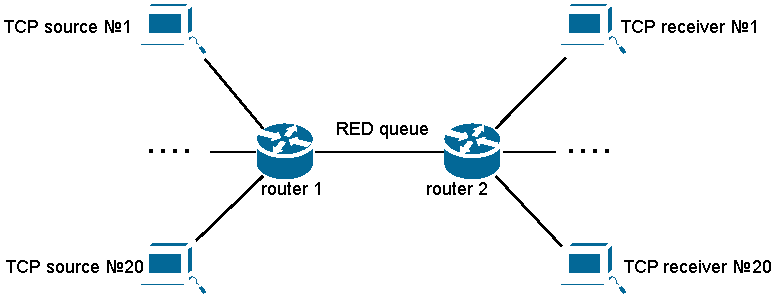
\includegraphics[width=0.7\textwidth]{topology}}
 \caption{Схема топологии моделируемой сети}
\label{ch3:fig1}
\end{figure}

Для данной топологии задали следующие параметры:

\begin{itemize}
\item между TCP-источниками и первым маршрутизатором дуплексные соединения 
	с пропускной способностью 100 Мбит/с и
  	задержкой 20 мс очередью типа DropTail;
\item между TCP-приёмниками и вторым маршрутизатором установлены
  	дуплексные соединения с пропускной способностью 100 Мбит/с и
  	задержкой 20 мс очередью типа DropTail;
\item между маршрутизаторами установлено симплексное соединение
  	($R1$--$R2$) с пропускной способностью 20 Мбит/с и задержкой 15 мс
  	очередью типа RED, размером буфера 300 пакетов; в обратную сторону~---
  	симплексное соединение ($R2$--$R1$) с пропускной способностью 15 Мбит/с и
  	задержкой 20 мс очередью типа DropTail;
\item параметры алгоритма RED: $q_{\min}=75$, $q_{\max}=150$, $q_w=0,002$, $p_{\max}=0.1$;
\item максимальный размер TCP-окна 32; размер передаваемого пакета 1000 байт;
  	байт; время моделирования~---100 единиц модельного времени.
\end{itemize}

\section{Моделирование сети в NS-2}
\label{chap3:sec1}

В имитационной модели TCP-приемники/источники, а также маршрутизаторы реализованы как стандартные узлы, данные передаются по протоколу FTP поверх TCP-Reno, 
для получения данных используются стандартные в программе средства, графики визуализируются в xgraph(для быстрого просмотра) и в GNUPLOT(для дальнейшего анализа).
Модифицированный NS-2 представлен в репозитории ~\cite{ns2-with-red}.

В файле nodes.tcl создаются узлы, задаются их соединения, а также настраиваются агенты и приложения на данные узлы. 
В файле queue.tcl на соеденение между маршрутизаторами накладывается RED, и описываются все его метрики. В файле TCP.tcl 
прописана функция для мониторинга таких метрик TCP, как cwnd, rtt и rtt\_var. В файле nam.tcl представлено создание nam файла для 
визуализации топологии. В файле timing.tcl задаются время моделирования. В файле finish.tcl описана процедура завершения. 
Все данные выводятся в каталог output, а графики в формате pdf c помощью скрипта GNUPLOT выводятся в каталог results. 
Все эти скрипты, запускающиеся с помощью головного файла main.tcl, представлены в Приложении.

Запустив первую модель с заданными параметрами, получили следующие результаты ~\ref{ch3:fig2}.

\begin{figure}[h!]
 \centerline{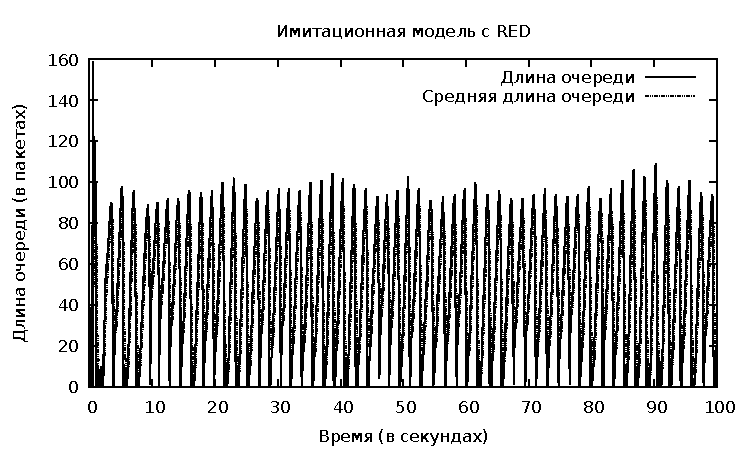
\includegraphics[width=0.7\textwidth]{queues}}
 \caption{График длины очереди и средней длины очереди на линке между маршрутизаторами}
\label{ch3:fig2}
\end{figure}

Как мы видим, в процессе моделирования очередь циклично варьируется от 0 до 100 пакетов.

Также провели модели для трех основных модификаций RED, GRED и ARED ~\ref{ch3:fig3, ch3:fig3.1}.

\begin{figure}[h!]
  \centering
  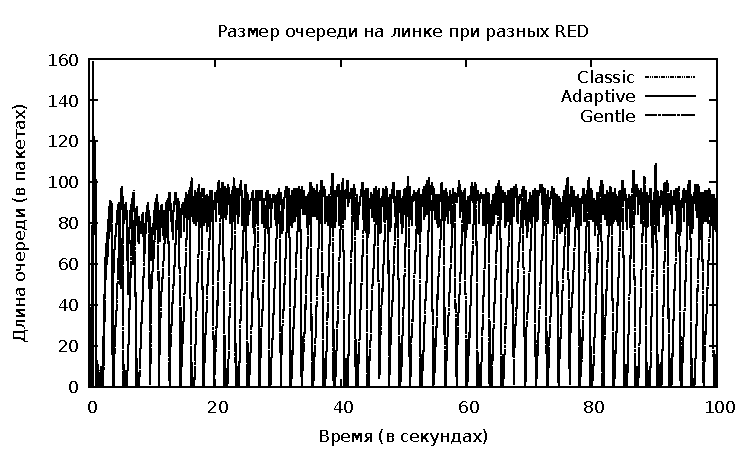
\includegraphics[width=0.7\textwidth]{red1queue}
  \caption{Очередь при основных алгоритмах RED}
  \label{ch3:fig3}
 \end{figure}

 \begin{figure}[h!]
  \centering
  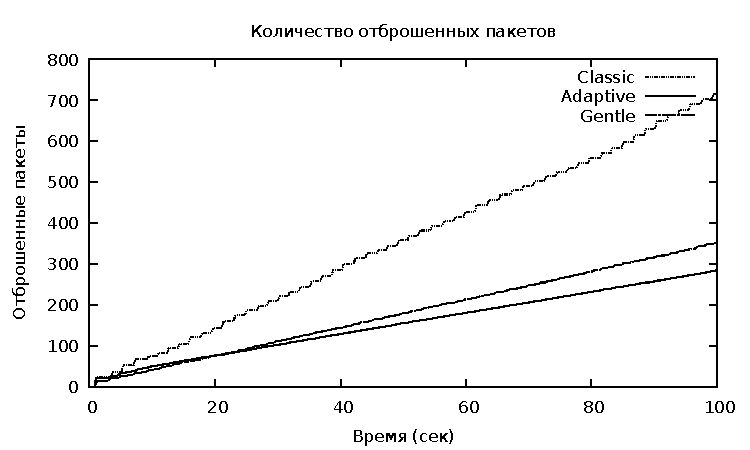
\includegraphics[width=0.7\textwidth]{reddrops}
  \caption{Количество отброшенных пакетов при основных алгоритмах RED}
  \label{ch3:fig3.1}
 \end{figure}
 
Как мы все можем наблюдать, адаптивный алгоритм сильно 
отличается от двух других алгоритмах при наших значениях, 
в нем длина очереди всегда выше минимального порога и 
держится приблизительно в промежутке от 80 до 100
пакетов. Это обьяснется его кардинально отличающимся 
алгоритмом, меняющим параметры в зависимости от сетевой нагрузки.
Монитроив также отброшенные пакеты, мы видим, что классический
алгоритм за это время отбросил в 2 раза больше пакетов чем
GRED, а ARED менее агрессивен по данному показателю, что логично
так как при данной модификации длина очереди всегда выше минимального
порога.

Проведя моделирования адаптивных модификаций, получили довольно похожие результаты ~\ref{ch3:fig4}.
Для модификации POWARED параметр $k=3$. 

\begin{figure}[h!]
  \centering
  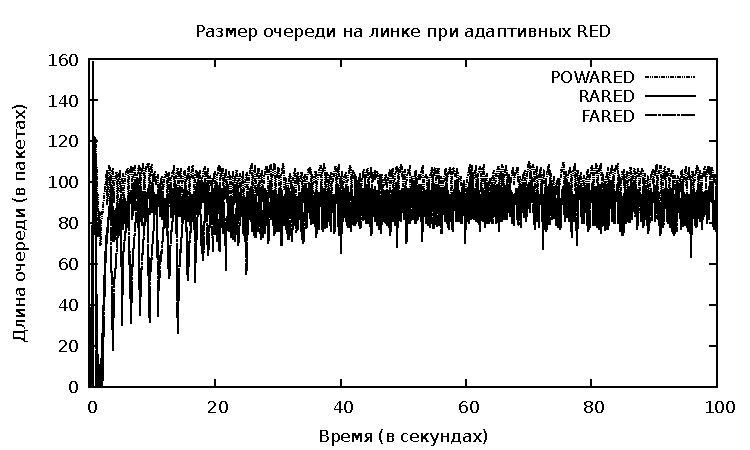
\includegraphics[width=0.7\textwidth]{red2queue}
  \caption{Очередь при адаптивных алгоритмах RED}
  \label{ch3:fig4}
 \end{figure}

Как мы наблюдаем, FARED и RARED доволно похожи и мы получаем
похожие значения, FARED в начале модели имеет больший диапазон
очереди, но максимальный размеры у них не отличаются, так как 
модификации отличаются только небольшим отличием числовых параметров.
А модификация POWARED при $k=3$ сохраняет больший размер очереди и вообще не опускается
ниже минимального порога. 

Для проведения сравнительного анализа различных нелинейных 
и кусочно-линейных алгоритмов, относящихся к семейству RED, 
было выполнено моделирование аналогичной топологии, время 
масштабировано до первых 25 секунд для большей наглядности. 
В результате получили следующие значения средневзвешенной экспоненциальной
очереди, см. рис. ~\ref{ch3:fig5}. В данном примере все алгоритмы, кроме DSRED, 
показали крайне схожие результаты обработки очереди. DSRED начинает 
отбрасывать пакеты более агрессивно из-за своего промежуточного значения $q_{mid}$.

\begin{figure}[h!]
  \centering
  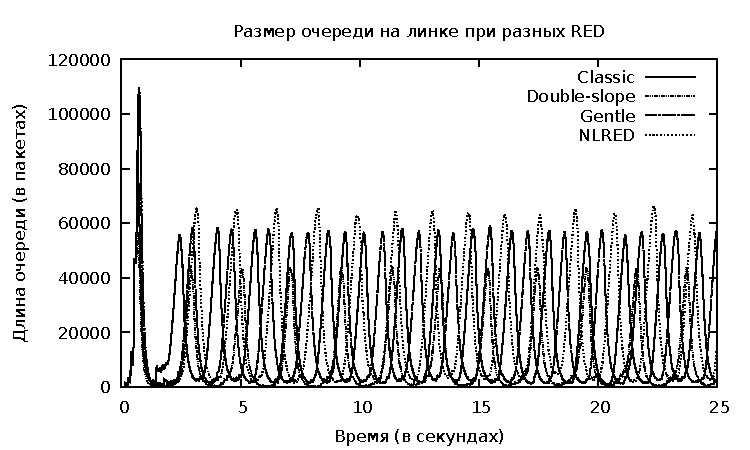
\includegraphics[width=0.7\linewidth]{red1}
  \caption{Длина очереди при разных алгоритмах RED}
  \label{ch3:fig5}
\end{figure}

\section{Моделирование сети в Mininet}
\label{chap3:sec2}

Модель в Mininet более сложная в реализации. В нем используются реальные виртуальные маршрутизаторы 
из класса LinuxRouter, описанных в ~\cite{mininet-repo} использованы коммутаторы для подсоединения к маршрутизаторам нескольких оконечных 
устройств, а также настроена ip-адресация для корректной работы программы. Для настройки очереди использован 
tc в которой реализованы только модийикации RED и ARED, передача пакетов происходит с помощью iperf3 и 
выводятся в json файл, из которой данные извлекаются с помощью shell скрипта из ~\cite{iperf3-plotter}. 
Также для моделирования программа обращаяется к ядру операционной системы, для того, чтобы изменить тип и размер
окна TCP. Для запуска на нескольких устройствах используются паралельные потоки. Для визуализации также используется GNUPLOT.
Также стоит учитывать, что при реальном моделировании, в отличие от имитационной, результаты могут отличаться при разных запусках,
в зависимости от многих факторов, как оперативная память компьютера, количество ядер процессора и т. д.  

В файле topology.py описаны создание топологии, двух маршрутизаторов, двух коммутаторов и соединеных 
с ними динамического количества оконечных устройств. В файле router.py описан класс LinuxRouter, 
используемых для данной сети. В файле utils.py описаны функции запуска iperf и мониторинга интерфейса с RED.
В файлах all.py и queue.py описаны функции для получения данных о метриках TCP и интерфейса с RED.
В файле main.py задана ip-адресация и созданы потоки для запуска модели.  

\section{Сравнение результатов в двух средствах моделирования}
\label{chap3:sec3}

Рассмотрим количество отброшенных пакетов в двух средствах. Как показано на Рисунках~\ref{fig:image1} и~\ref{fig:image2}, 
поведение системы в NS-2 и Mininet имеет значительные различия в отношении количества отброшенных пакетов.

\begin{figure}[ht]
    \centering
    % Первый рисунок
    \begin{minipage}[b]{0.45\textwidth}
        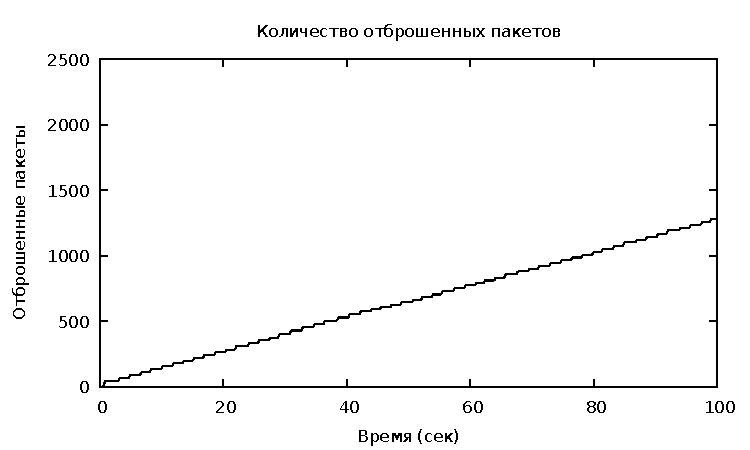
\includegraphics[width=\textwidth]{drops_NS2}
        \caption{Отброшенные пакеты в NS-2}
        \label{fig:image1}
    \end{minipage}
    %\hfill % Добавляет пробел между изображениями, если это необходимо
    % Второй рисунок
    \begin{minipage}[b]{0.45\textwidth}
        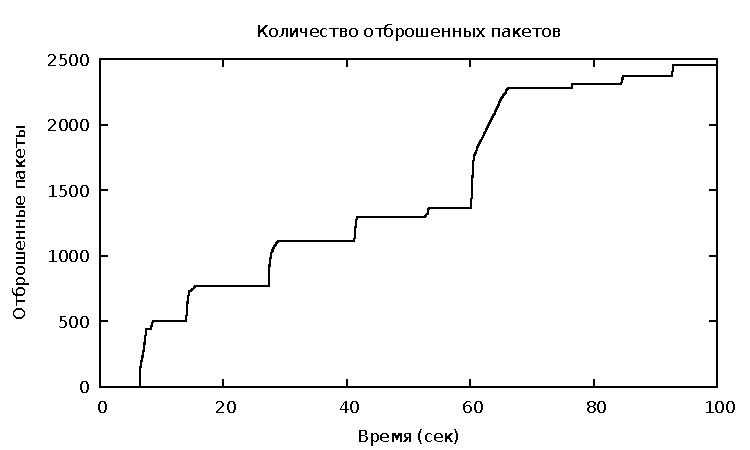
\includegraphics[width=\textwidth]{drops_mininet}
        \caption{Отброшенные пакеты в mininet}
        \label{fig:image2}
    \end{minipage}
\end{figure}

Как мы видим, при натурном моделировании отбрасываются больше пакетов, 
а более плавное изменение графика в NS-2 обьяснется тем, что мониторинг
данных происходит с большей частотой.  



%%% Local Variables:
%%% mode: latex
%%% coding: utf-8-unix
%%% TeX-master: "../default"
%%% End:
